%%CHAP. Ocean

%%-- SW06 experiment 
\begin{figure}
\centering
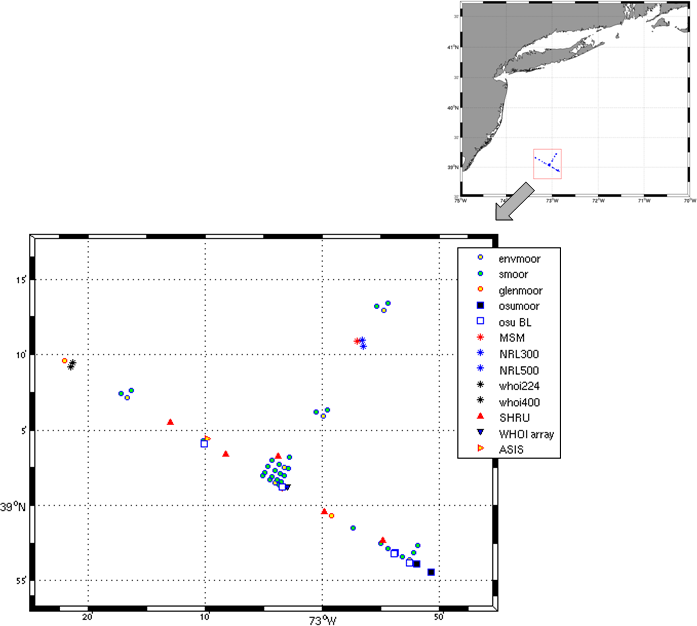
\includegraphics[width=\textwidth]{moorings_site.png}
\caption{Map of SW06 experiment site and the locations of the environment and acoustic moorings}\label{fig:mooring}
\end{figure}

\begin{figure}[h]
\centering
  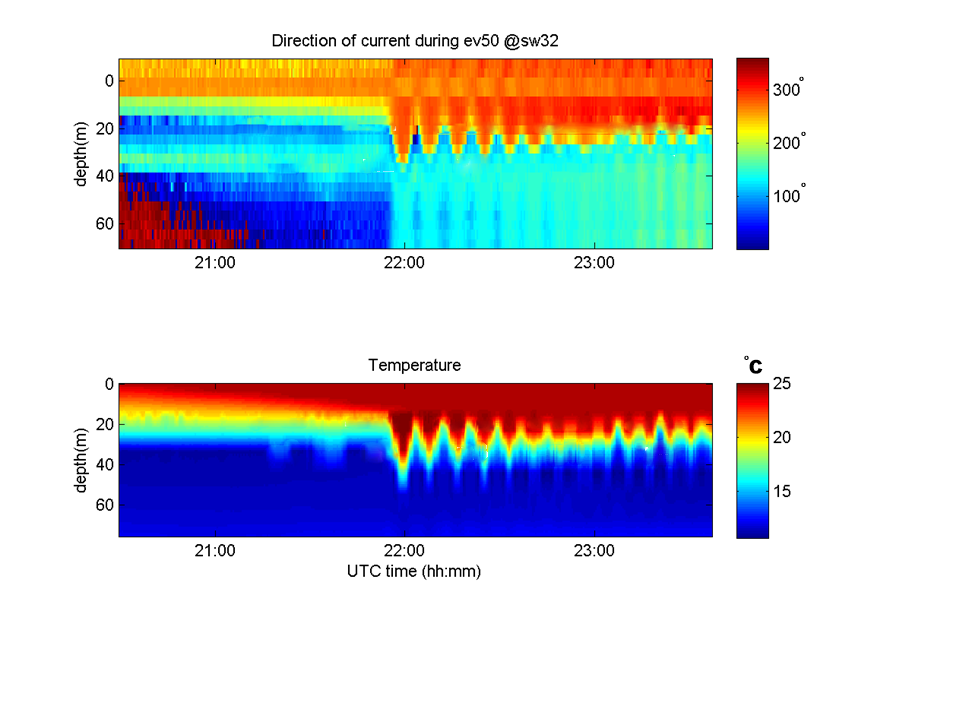
\includegraphics[width=\textwidth]{sw32adcp_temp_1.png}\\
  \caption{Current data record by ADCP at mooring SW32 during event 50 in SW06 experiment (upper panel) and  temperature data at the same location. }
  \label{fig: sw32adcp_temp}
\end{figure}

\begin{figure}[h]
\centering
  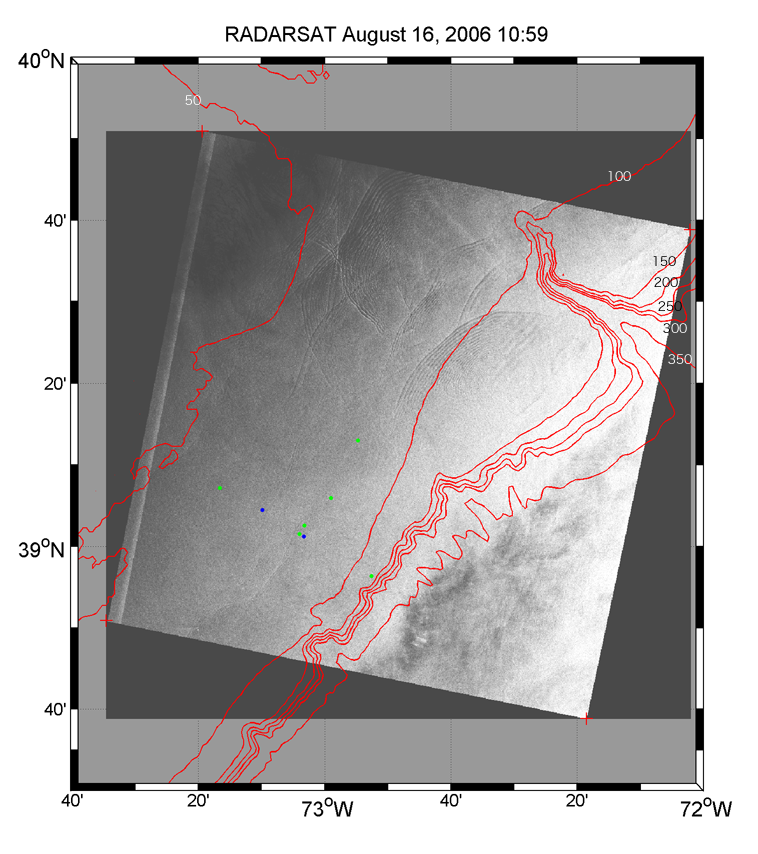
\includegraphics[width=0.8\textwidth]{RADARSAT.png}\\
  \caption{Image of SW06 experiment site taken by the Canadian RADARSAT satellite on 16 August, 2006.  }
  \label{fig:radarsat}
\end{figure}
%
%\begin{figure}[h]
%\centering
%  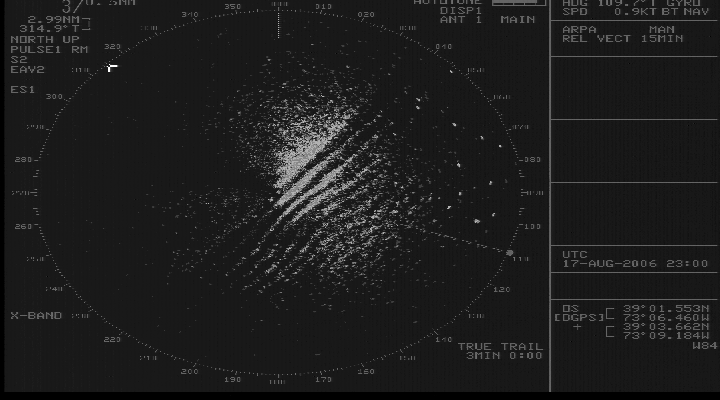
\includegraphics[width=0.8\textwidth]{20060817230014GMT.png}\\
%  \caption{R/V Oceanus radar image shows the internal wave packet of Event 50 in SW06 at GMT 23:00, Aug 17th. }
%  \label{fig:oceanus_radar}
%\end{figure}

\begin{figure}[h]
\centering
  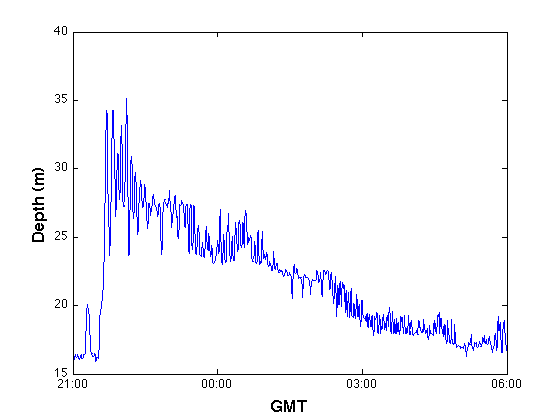
\includegraphics[width=0.8\textwidth]{sw54_aug17_thermocline_18C_long.png}\\
  \caption{Depth of  $18^oC$ degree thermocline on Aug. 17, 2006, recorded on WHOI Sharp VLA (SW54)}
  \label{fig:sw54_aug17_thermocline_18C_long}
\end{figure}

\begin{figure}[h]
\centering
  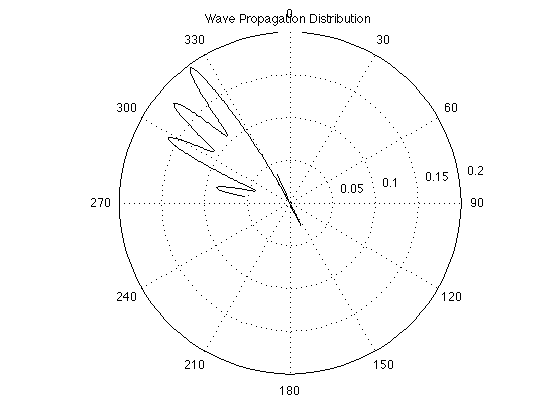
\includegraphics[width=0.8\textwidth]{IW_dir.png}\\
  \caption{Angular distribution of the direction of the internal wave recored during SW06. }
  \label{fig:IW_dir}
\end{figure}


\begin{figure}[h]
\centering
  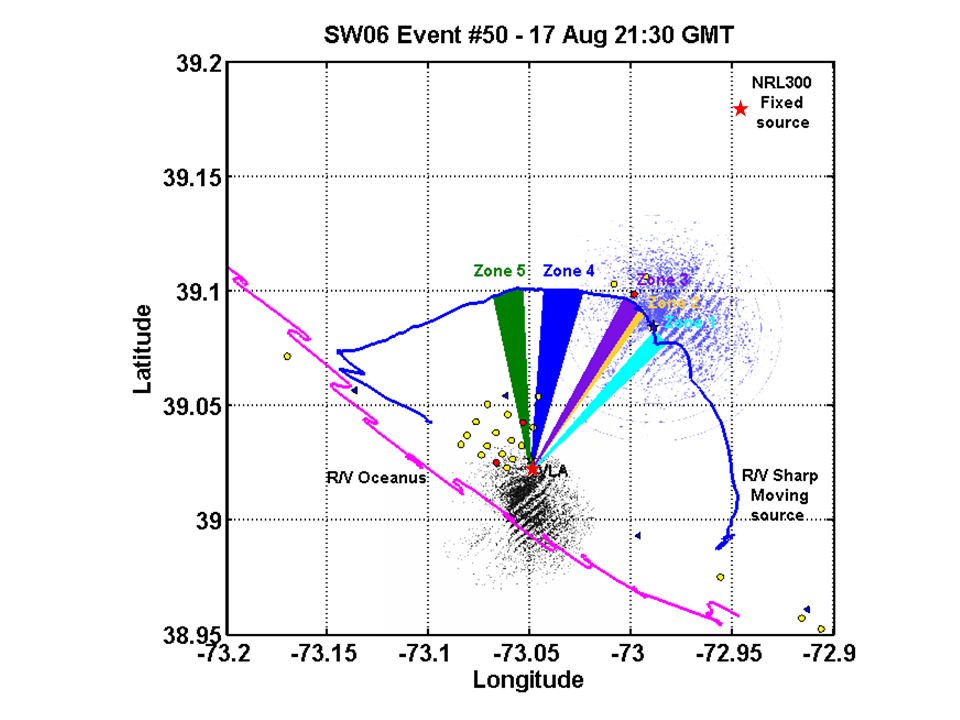
\includegraphics[width=0.8\textwidth]{ship_track_radar_report.png}\\
  \caption{Diagram showing the fixed acoustic source(NRL300), receiver array (Shark VHLA) and the semi-circular track of R/V Sharp the IW event 50. Zone 1~5 represent the location of J15 in the time periods when it was transmitting in event 50.}
  \label{fig:ship_track_radar}
\end{figure}

